\documentclass[a4paper,11pts]{article} 
% A4: 210 × 297 mm   carta: 216 × 279 mm
\usepackage[a4paper]{geometry}
\geometry{top=2.54cm, bottom=2.54cm, left=2.54cm, right=2.54cm}
%2.54cm (1in) a todos lados segun las normas apa

\usepackage[utf8]{inputenc}
\usepackage[spanish]{babel} % espanol
\usepackage{float}
\usepackage{color}
\usepackage{colortbl}

\usepackage[bookmarks = true, colorlinks=true, linkcolor = black, citecolor = black, menucolor = black, urlcolor = black]{hyperref}


\usepackage{graphicx} % graficos
\graphicspath{ {./images/} }
\usepackage{setspace}%interlineado agrega:
% \doublespacing \onehalfspace \singlespace \spacing{x}
\spacing{1.5}
\pagestyle{headings}
%\setlegtth{\parindent}{<distancia>}
\usepackage{subfig}

\usepackage[backend=biber]{biblatex}
\bibliographystyle{te}

\bibliography{referencias}


\begin{document}

	\setcounter{page}{0}
\begin{titlepage}

\begin{table}[t]
\centering
\begin{tabular}{ p{3cm} p{8.5cm} p{3cm} }
	\begin{flushleft}
\includegraphics[width=2.4cm]{logo_poli.png}\end{flushleft} &



	\begin{center}
	República Bolivariana de Venezuela\\
	Universidad Nacional Experimental Politécnica “Antonio José de Sucre”\\
	Vice Rectorado Barquisimeto \\
	Departamento de Ingeniería Electrónica\\  

%***************************************************
%************** aqui va el titulo ******************
%***************************************************

	\vspace*{65mm}
	\begin{LARGE}Herramienta computacional para el análisis de la vibración en motores eléctricos alimentada mediante datos de una simulación digital\end{LARGE}
	\vspace*{75mm}
	\end{center}



	& \begin{flushright}
\includegraphics[width=1.7cm]{logo_electronica.jpg} \end{flushright}
\end{tabular}

\begin{flushright}
Integrantes:\\


Gerardo Alfonzo Campos Fonseca\\ 
V. 27085179\\
José Andrés Cortez Teran\\
V. 26540824\\

\vspace*{3mm}
Tutor: Dra. Luisa Escalona\\

\end{flushright}
\vspace*{5mm}

\begin{center}Barquisimeto, Abril del 2021\end{center}
\end{table}
\end{titlepage}



	%\newpage
	%\tableofcontents
	%\newpage

	%Capitulo 1
	\begingroup
		\let\clearpage\relax
		\setcounter{page}{1}

\begin{center}
	\section{Planteamiento del problema}
\end{center}


%\subsection{Descripción del problema}

	En la actualidad se vive un crecimiento exponencial a nivel industrial dadas las altas demandas de alimentos e insumos de toda clase, esto es posible, entre otras cosas, gracias al motor eléctrico, este es un artefacto que transforma la energía eléctrica en energía mecánica (movimiento), de manera que puede impulsar el funcionamiento de una máquina y son utilizados ampliamente en: Bombas para Agua, Bombas Industriales, Mezcladoras, Molinos, Correas Transportadoras, Zarandas, Cortadoras, Ventiladores, Grúas, y en todo proceso que involucre movimiento.\\
	Adicional a su versatilidad, existen otros factores como las grandes perdidas (horas, insumos,dinero, etc) qué ocasionan una parada de emergencia en una planta, por los cuales se considera de vital importancia que los motores se encuentren completamente operativos y funcionales. y para procurar su buen estado y funcionamiento, se deben realizar mantenimientos.\\



	Existen diferentes tipos de mantenimiento, entre ellos están: 
	\begin{itemize}
		\item Correctivo: se espera que ocurra una falla para
	reparar o cambiar un equipo. Esto puede degradar la vida útil del equipo y debido a que la falla puede ocurrir en cualquier momento, usualmente se produce un paro en la linea de producción, por lo tanto este tipo de mantenimiento suele y debe ser evitado.

		\item Preventivo: para evitar una falla mayor se detiene la maquinaria para hacer un mantenimiento preparado con anticipación, se inspecciona la maquinaria y se remplazan las piezas propensas a dañarse. Este tipo de mantenimiento en algunas circunstancias es más que suficiente pero en el caso de los rodamientos puede ser contraproducente.

		\item Predictivo: se pronostica cuando una falla esta a punto de ocurrir; a través de mediciones y estudio se prevé cuando un desperfecto esta a punto de ocurrir y de esta forma se realiza una mejor planificación. Cabe resaltar que este tipo de mantenimiento puede dar información acerca del origen y la gravedad de las averías.
	\end{itemize}

	En el caso de los motores eléctricos, como dice Dr.S. J. Lacey (~\cite{Lacey}), el mantenimiento preventivo tiene muchas desventajas dado que existen tanto problemas de índole mecánico como administrativo y monetario como lo pueden ser los altos costos de reemplazo dado que las partes se reemplazan muy pronto, el riesgo de pérdida completa dado un error humano, instalación de una pieza defectuosa, además de la posibilidad de generar daño o una incorrecta instalación de la misma, y por ultimo, el hecho de que las piezas reemplazadas pueden tener muchos años de vida útil.\\
	
	Por otro lado, el mantenimiento predictivo ofrece mas control sobre las variables mencionadas y aunque no evita las posibilidades de error humano, si permite reaccionar a este; adicionalmente, se deben considerar las altas pérdidas y retrasos, sumadas a las dificultades administrativas, que generan las paradas periódicas de la planta.\\

	Por las razones expuestas surge la necesidad de reconocer las fallas ya que los factores que las causan al estar bajo continuo monitoreo, principio del mantenimiento predictivo, se pueden atenuar según los estudios realizados por J. Kammermann, I. Bolvashenkov, S. Schwimmbeck, y H.-G. Herzog (~\cite{Kammermann}) la media de la probabilidad de fallas en máquinas de inducción permanece al nivel de los años 70 ($10^{-6}/hour$) y está altamente relacionada a la falla de los rodamientos, y que un 59\% de las fallas son causadas por los rodamientos, esto es debido a que son piezas sometidas a mucho estrés mecánico, permiten soporte y asimismo necesitan tener poca fricción. Por esta razon, su principal falla es el desgaste, de igual forma se presentan otras fallas estructurales que generan vibraciones. Cabe resaltar que todas las fallas mecánicas generan vibración sin importar su relación con los rodamientos y lo hacen a distinta frecuencia ($f$). \\


	Por lo expuesto, es de suma importancia el estudio de la vibración, para la que se suele implementar un acelerómetro y con un estudio de la frecuencia se puede obtener la causa y la magnitud de la falla y de esta forma programar su reparación.\\
	Debido a que esta evaluación debe ser realizada en cada rodamiento y acople o extensión del motor y dadas las mediciones que se deben realizar por unidad (motor y acoples) y por la gran cantidad de unidades existentes a nivel industrial, es virtualmente imposible el estudio con un acelerómetro convencional( a pesar de que la medición no sea un proceso muy largo y los cálculos y evaluaciones sean realizados posteriormente). Sumado a esto, las industrias suelen poseer medidas y controles sanitarios, aumentados por la pandemia actual, que no permiten el constante monitoreo de la planta significando esto la imposibilidad de implementar este tipo de mantenimiento de forma manual, por lo cual se debe recurrir a un sistema de automatización capaz de medir las vibraciones en todos estos equipos que, a su vez, permita el estudio de estos datos de forma remota. \\

	


		
%\subsection{solución}

%Para llevar a cabo lo expuesto anteriormente %en el planteamiento del problema
Para esto, se plantea la implementación de un sistema capaz de tomar datos de forma continua y enviarlos a un servidor el cual permita el almacenar, estudiar y muestrear la información en distintos niveles de profundidad, con respecto al análisis realizado.\\
Para esto se plantea una simulación digital, diagramada en la figura \ref{fig:diagrama}, que constara de un análisis estadístico para obtener las medidas típicas de un acelerómetro en motores eléctricos con distintos niveles de daños, esta data permitirá, después de ser almacenada en una base de datos y procesada, generar 3 niveles de análisis:\\
\begin{itemize}
\item La vista principal, permitirá observar una cantidad especifica de motores, simbolizando los existentes en una planta o piso, y su estado general.

\item La vista especifica, dará la información actual e histórica referente a un único motor previamente seleccionado.

\item La vista exhaustiva se refiere a un análisis en frecuencia de la vibración de un motor especificado con anterioridad, con la finalidad de permitir al operador o ingeniero encargado determinar la causa de las posibles averías.
\end{itemize}


Y finalmente, toda esta información y opciones se mostrarían a través de una pagina web para facilitar su acceso.

\begin{figure}[htb]
\centering
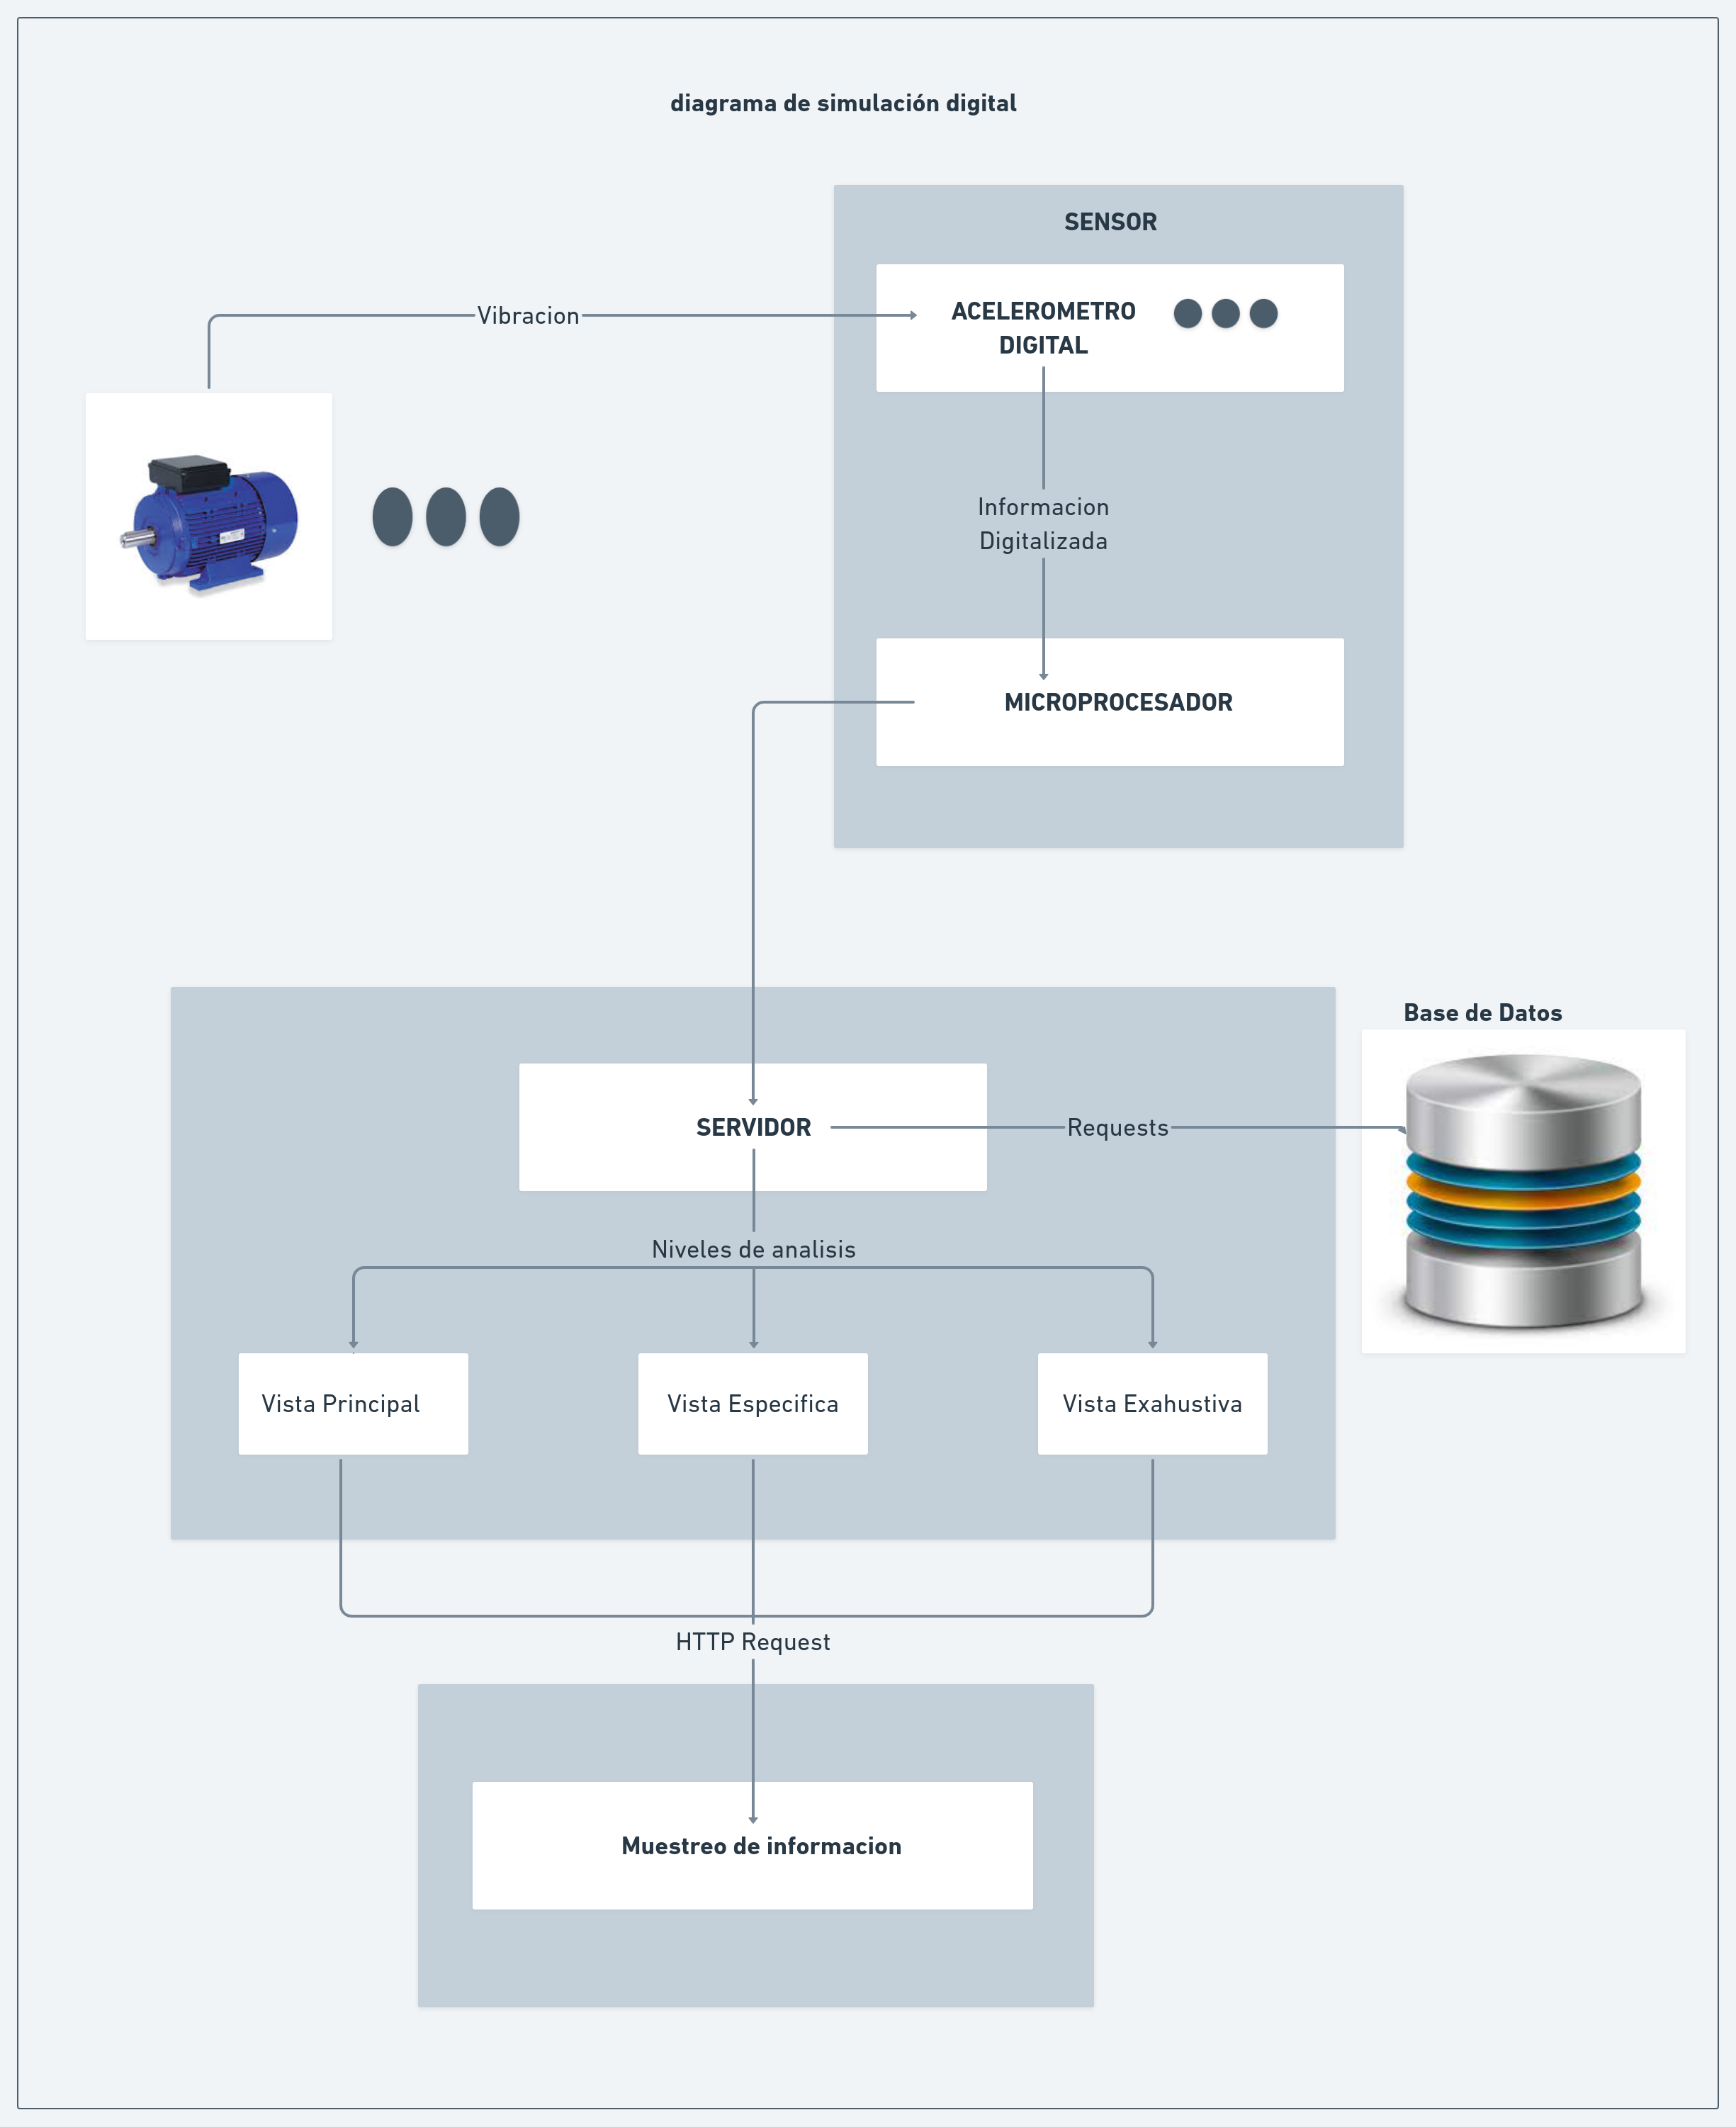
\includegraphics[width=15cm]{Diagrama_sensorica.png}
\caption{Diagrama de la simulación digital}
\label{fig:diagrama}
\end{figure}


	
	\endgroup
	
	\subsection{Objetivos de la investigación}

\subsubsection{Objetivo general}
	\begin{enumerate}
		\item  Desarrollar la simulación digital del monitoreo de la vibración en motores eléctricos mediante un acelerómetro, con la finalidad de hacer diagnósticos predictivos.
	\end{enumerate}
	
\subsubsection{Objetivos específicos}

	\begin{enumerate}
		\item Justificar la escogencia de las herramientas y lenguajes a utilizar en las diferentes etapas que requiere la simulación. (José cortez y Gerardo Campos)

		\item Elaborar un análisis estadístico de motores con distinto grado de daño que establezca la distribución de la salida de acelerómetro digital. (José cortez)

		\item Elaborar una base de datos con la cual se establezcan el análisis  en simulación digital. (José cortez y Gerardo Campos) 
		
		\item Realizar análisis de fallas en frecuencia, a partir de la salida de la distribución del acelerómetro. (Gerardo Campos)

		\item Mostrar la información solicitada de acuerdo al nivel de análisis seleccionado. según sea: Vista Principal, Vista Específica o Vista Exhaustiva. (José cortez y Gerardo Campos)

		\item Comprobar los resultados de la simulación digital. (José cortez y Gerardo Campos)
	\end{enumerate}

	
	\subsection{JUSTIFICACIÓN E IMPORTANCIA}

Para prevenir las fallas mecánicas que ocurren en los motores, por el deterioro
y desgaste de los rodamientos, estos se deben tener bajo constante monitoreo
para poder efectuar un mantenimiento puntual que elimine dichos peligros. De
esta forma el mantenimiento predictivo es la clave para mejorar la vida útil,
funcionamiento y planificación de todo proceso especialmente a niveles
industriales, donde la cantidad de motores eléctricos es bastante elevada
por lo cual la automatización del proceso es crucial.

Sin embargo, dado los altos costos que implican realizar una automatización y
en especial a escalas industriales se suele hacer una simulación o una
emulación para estudiar y obtener el modelo más preciso, gracias a la facilidad
de manipular con mayor eficacia los diseños y conocer su comportamiento real
sin necesidad de construirlo, antes de realizar la implementación y todo el
proceso que esta conlleva.

Habiendo expuesto la importancia del mantenimiento como también la de realizar
simulaciones, se justifica el hecho de realizar el desarrollo del trabajo aquí
propuesto el cual permita emular el comportamiento y las salidas de un
acelerómetro, como también otorgar las herramientas necesarias para
realizar un mantenimiento predictivo, y de esta forma estudiar a
profundidad su estado actual como también su evolución histórica. Todo esto
sumado a las facilidades de portabilidad que ofrece un sistema Web, facilitando
la revisión constante sin las dificultades de los protocolos de acceso y
sanidad usuales en las plantas industriales.


	\printbibliography[title={\centering{Referencias Bibliográficas}}]

\end{document}
